\section{Introduction}\label{sec:introduction}
An emerging trend in algorithmic stock trading is the use of automatic search through the Web, the blogosphere, and social networks for relevant information that can be used in fast trading, before it appears in the more popular news sites~\cite{Delaney2009,ALPHA2014,AlphaFlash,mitra2011handbook,latar2015robot}. Similarly, intelligence, business and politics analysts are scanning online sources for new information or rumors. While new items are often rebloged, retweeted and posted on a number of sites, the goal is to find the information, somewhere, as fast as possible before we gradually loose the interest in them. %There is no benefit in seeing more copies of the same news item, rumor, etc.

Such a search is an example of a fundamental search and detection problem in dynamic, distributed massive data repository.  Data is distributed among a large number of nodes, new items appear in individual nodes, and items may propagate (copied) to neighboring nodes on a physical or a virtual network.  The goal is to detect at least one copy of each new item as soon as possible. The search application can probe any node in the system, but it can only access and process a few nodes at a time. 
To minimize the time to find new items, the search application needs to optimize the schedule of probing nodes, taking into account (i) the way items get distributed among the nodes (to see where to probe), and (ii) how items' freshness (or relevance) decay over the time (to avoid the worthless probes).

% the likelihood of nodes to generate new items, to receive new items, to propagate items to other nodes, and how yet undiscovered items loose their impact/value over the time.

Another application that faces a similar search problem is processing security raw data (e.g. gathered security raw footages that need to be processed). Ideally, given limited resources compared to the huge size of the data, an schedule for processing (probing) different raw-dataset has to minimize the value of missing information (assuming newer information are more valuable than older ones).

To formally define our search problem, {\probname} we need the following definitions.

\begin{definition}[Generating System]
 Suppose $U=\set{1,\ldots,n}$ is a universal set of elements, $\F$ is a family of subsets of $U$, and $\pi:\F \rightarrow [0,1]$. We call the elements of $\F$ \emph{\ins} of $U$. A \emph{generating system} $\sys = (U, \F,\pi)$ is an infinite time system that at each time step generates a random sample $\S\subseteq\F$, such that a set $S\in \S$ is randomly chosen with probability $\pi(S)$. Thus, $\sys$ generates a sequence $\S_1,\S_2,\ldots$ where each $\S_t$ is a sample of {\ins}s generated at time $t$. An \emph{item} $i_{t,S}$ is a \emph{copy} of the {\ins} $\S$ generated at time $t$.
\end{definition}

\begin{definition}[Schedule]
 For a positive integer $c$, a \emph{$c$-schedule} for a generating system $\sys=(U,\F,\pi)$ is a probability distribution $\p$ over $U^c$. Probing via  a schedule $\p$ is an infinite process, such that at any time step, we choose (up to) $c$ nodes chosen randomly according to $\p$ to probe. We say an item $i_{t,S}$ is \emph{caught} at time $t'\geq t$, if $\p$ probes a node of $\S$ at time $t'$, for the first time after time $t$.
\end{definition}

\begin{definition}[Cost]
Suppose $\sys =(U,\F,\pi)$ is a generating system and $\theta\in[0,1]$ is the decaying factor. The \emph{freshness} of an \emph{uncaught} item $i_{t,S}$ at time $t'\geq t$ is $\theta^{t'-t}$. Define the \emph{load} of $\sys$ at time $t$, denoted by $L_\sys(t)$, as a r.v. that equals to the sum of the freshness of uncaught items at time $t$. The $\theta$-\emph{cost}, or \emph{cost} in short, of a schedule $\p$ is defined as $\E_{t}(L_\sys(t))$. We denote the cost of $\p$ by $\cost{\p}$.
% = \sum_{S\in\F}\frac{\pi(S)}{1-\theta(1-\p(S))}.$$
\end{definition}

\begin{definition}[\probname]
 The goal in a $(\theta,c)$-{\probname} ($(\theta,c)$-PHSP) for a generating system $\sys$ is to find  a $c$-schedule with the minimum $\theta$-cost. We call a schedule \emph{optimal} if it has the minimum cost.
\end{definition}

Note that in $(\theta,c)$-PHSP, the parameter $\theta$ tunes our interest in older items. For instance, if $\theta=0$ then each item will stays in the system only for one step as its freshness disappears immediately. So, ideally, a schedule should catch as many \emph{new items} (generated in the current time step) as possible (\ahmad{This can be viewed as a multi-arm bandit problem where each element $u\in U$ represents a bandit, and the score we get total freshness of the items that we catch by probing $u$}). In the other extreme, if $\theta=1$, an ideal schedule should consider all the items for catching, regardless of their age.

Although we introduced the $(\theta,c)$-PHSP as a search problem, it gives us a very general framework for asking ``social network'' problems, such as finding the most \emph{influential}~\cite{borgs2014maximizing,kempe} or the most \emph{central}~\cite{yoshida2014almost} set of nodes:
 

\begin{itemize}
 \item {\bf Influence Maximization:} Given a social social network $G=(U,E)$ and a cascade model for propagation on $G$, the goal is to find a set of $c$ nodes that maximizes the size of the cascade seeded at these nodes. In \cite{borgs2014maximizing} they introduced the notation of random hyper-edge, a random subset of nodes sampled according to a distribution $\pi'$. They showed that for a given set of nodes $N$, the influence of $N$, $\sigma(N)$, is
 \begin{equation}\label{eq:infmax}
\sigma(N) = n\cdot \pr_{S\sim \pi'} (N \cap S \neq \emptyset),
 \end{equation}
 where $n$ is the number of nodes in $G$. Thus, a set $N\subseteq U$ of size $c$ has the maximum influence if and only if it maximizes $\Pr_{S\sim \pi'}(N\cap S\neq \emptyset)$. 
 
 Now, let $\sys=(U,\F,\pi)$ be the generating system in which $\F$ is the family of all subsets of $U$ and $\forall S\in \F: \ \pi(S) = \pi'(S)$. Suppose $\p$ is an optimal $c$-schedule of the $(0,c)$-PHSP for $\sys$. Note that without loss of generality, since $\theta=0$, we can assume that $\p$ always  probes a \emph{fixed} set of $c$ nodes, $N$, that minimizes the total missing freshness, i.e., the total probability of the items that $\p$ does not catch at a time step; this is because after each step all the items are removed and the system resets. So, we have
 $$\cost{\p} = \min_{N'\subseteq U: |N'|=c} 1 - \Pr_{S\sim \pi'}(N'\cap S\neq \emptyset) = 1 - \Pr_{S\sim \pi'}(N\cap S\neq \emptyset),$$
 and thus, $\Pr_{S\sim \pi'}(N\cap S\neq \emptyset)$ is maximized and $N$ is a set of $c$ nodes with maximum influence. 
 Therefore, the Influence Maximization problem can be translated into a proper $(0,c)$-PHSP.
 
 
 \item {\bf Set Centrality Maximization\cite{yoshida2014almost}:} 
 In~\cite{yoshida2014almost} the problem of finding a set of $c$ nodes with maximum centrality was studied, for two different centrality measures (betweenness and coverage). Here, we see how finding a set (of size $c$) with maximum betweenness centrality can be presented as a $(0,c)$-PHSP (the results hold for coverage centrality as well using the proper hyper-edges introduced in~\cite{yoshida2014almost}).
 
 In a network $G=(U,E)$, the betweenness centrality of a set $N\subseteq U$ is defined as\footnote{In some other works, different normalizing factors are considered. However, without loss of generality we let the normalizing factor to be $\frac{1}{n(n-1)}$.}
 $$C(N) = \frac{1}{n(n-1)}\sum_{u,v\in V} \frac{\tau(u,v; N)}{\tau(u,v)}$$
 where $\tau(u,v)$ is the number of shortest path from $u$ to $v$, and $\tau(u,v;N)$ is the number of shortest path from $u$ to $v$ that pass any node in $N$. The goal is to find a set of $c$ nodes with maximum betweenness centrality. Suppose $\pi'$ is a distribution over the shortest paths of $G$, where each shortest path $P_{u,v}$ is chosen with probability $\frac{1}{n(n-1)\tau(u,v)}$. If $\texttt{in}(P)$ denotes the internal nodes of the path $P$, it has been shown~\cite{yoshida2014almost,mattoe?} the most central set of $c$ nodes is a set $N$ such that 
 $$N\in \argmax_{N'\subseteq U: |N'|=c} \pr_{P\in\pi'}(\texttt{in}(P)\cap N' \neq \emptyset).$$
 
 
Let $\F$ be the family of sets $S$ where each $S$ is the internal nodes of a shortest path in $G$, and define 
 $$\forall S\in\F : \ \pi(S)=\sum_{\text{shortest path} P: \texttt{in}(P)=S} \pi'(S).$$
Now, if $\sys=(U,\F,\pi)$ is a generating system, using a similar argument as above, we can assume that an optimal $c$-schedule for its $(0,c)$-PHSP probes a fixed set of $c$ nodes, $N$, that also has the maximum centrality.
\end{itemize}

% Obviously, the $c$-PHSP is an NP-hard problem as it reduces to other NP-hard problems (e.g., influence maximization). However, these reductions are to the cases where $\theta=0$ and general positive integer $c$. 
In this work, we focus on $(\theta,1)$-PHSPs. In the following sections, we first study the $(\theta,1)$-PHSPs and provide different methods for finding the optimal schedule. We also show how in a generating system $\sys=(U,\F,\pi)$ our method works even if we do not have access to $\F$ or $\pi$, using only the samples of {\ins}s generated by $\sys$. Next, we show the scalablity of our method in using the MapReduce framework. Finally, we apply our method to a variety of real networks, and the results of our experiments demonstrate the practicality and optimality of our solution. 

% $\theta \in (0,1)$ and $c=1$ (see Figure~\ref{fig:square}) and show that it is possible to find  an optimal probing schedule for $1$-PHSP in $\sys=(\F, \pi, \theta)$, efficiently, and without having any prior information on distribution of items, i.e., knowing $\pi$ is not assumed in our algorithm.


% \begin{figure}[h!]
%   \centering
%     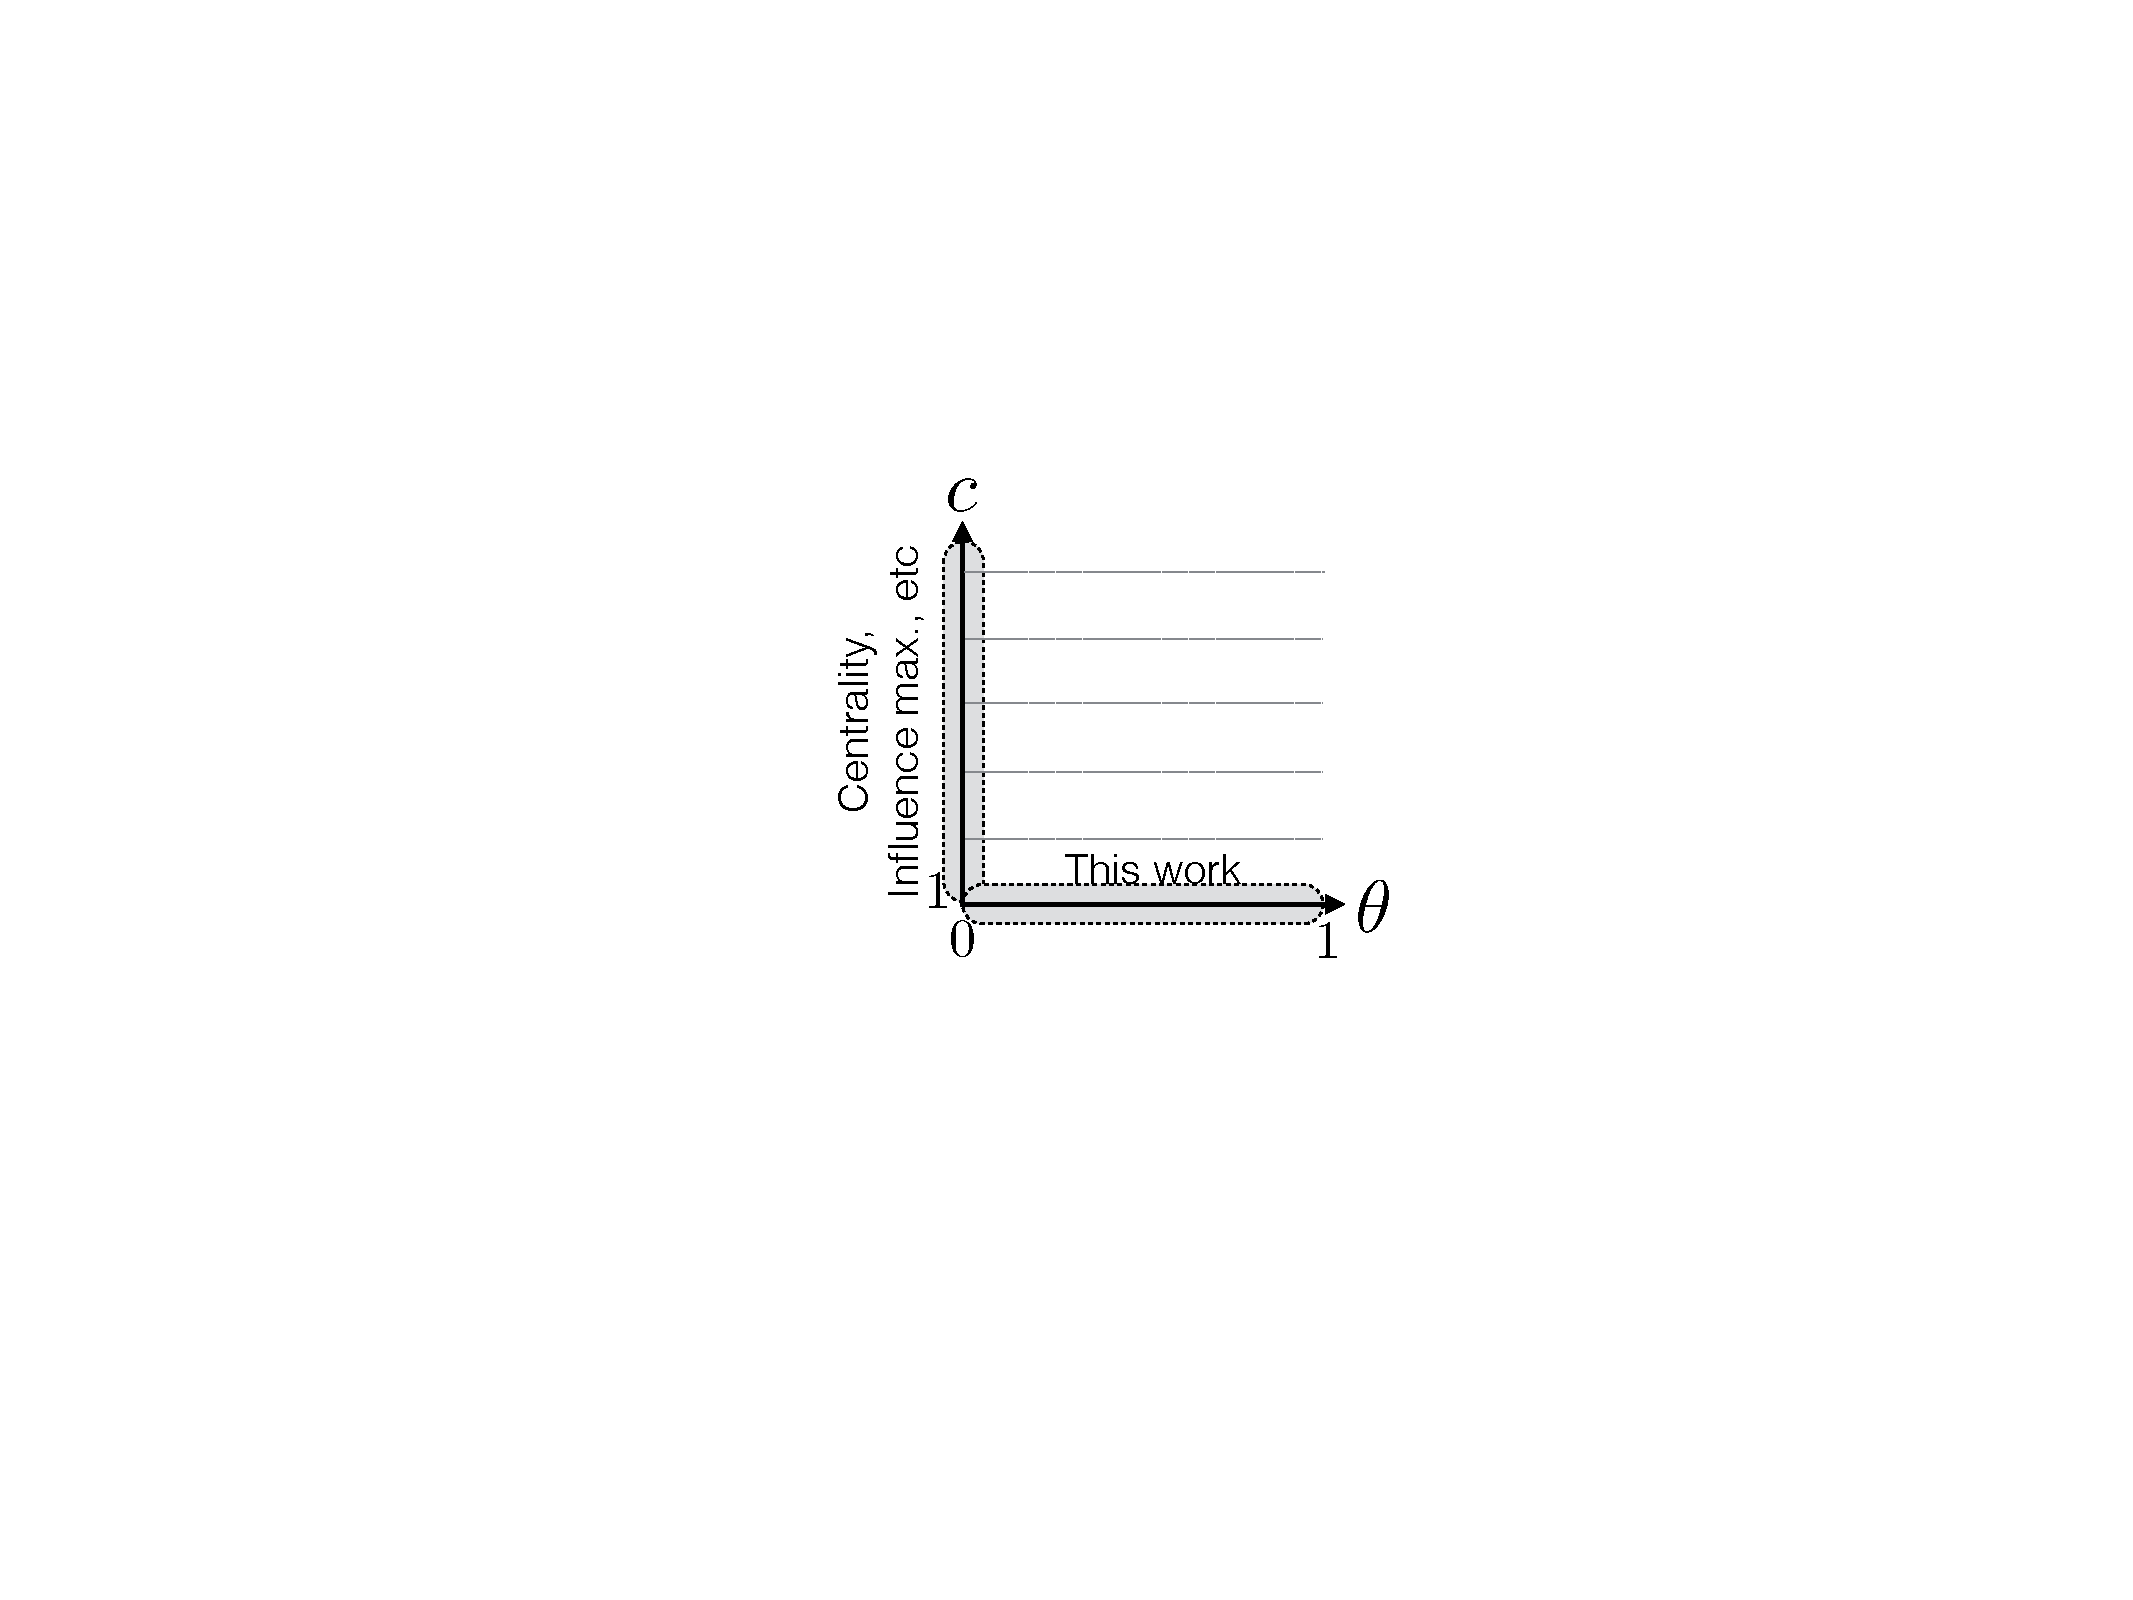
\includegraphics[width=0.25\textwidth]{figures/square.pdf}
%  \caption{}
% \label{fig:square}
% \end{figure}

% Specifically, our goal is to provide an efficient tool for a user who does not have a prior information on the generation and distribution of items in the network. We focus on simple, memoryless probing schedules that are easy to compute and require minimum storage. Our solution consists of two major components. We first develop an efficient algorithm for computing a near optimal schedule. Then, using Hoeffding's inequality, we show prove having only to a family $\M$  of \emph{sampled} informed set gathered during a very short amount of time (during $O(\log(n))$ time intervals, where $n$ is the number of nodes), without having access to $\S$,  $\pi$, or the network topology, we are still able to apply our method accurately. 


